\section{Cámara}

Para la cámara he utilizado una de tipo \textit{Target}, cuya posición comienza en la izquierda de la escena.

Voy a dividir en dos subsecciones la animación del propio movimiento de la cámara y del seguimiento de los objetos de la escena:

\subsection{Movimiento de la cámara}

Cabe destacar que aparte del movimiento de izquierda a derecha en la escena, he animado un tercer movimiento final que hace que la cámara se ponga justo detrás de la espada, para visualizar su movimiento y el recorrido que hace el coche.

\bigskip

Por tanto, para realizar la animación de la cámara hacen falta los siguientes \textit{keyframes}:

\begin{itemize}
    \item \textbf{Instante 65: }La cámara se encuentra a la izquierda de la escena.
    \item \textbf{Instante 90: }La cámara se encuentra a la derecha de la escena.
    \item \textbf{Instante 125: }La cámara se encuentra en la posición que en el instante anterior, está esperando a que la espada suba junto a la plataforma.
    \item \textbf{Instante 150: }La cámara se encuentra detrás de la espada, mostrando el movimiento de esta y del coche junto a sus ruedas.
\end{itemize}

\bigskip

Las curvas de animación son las siguientes: 

\begin{figure}[H]
    \centering
    % curvas de animacion
    \begin{subfigure}[t]{0.32\textwidth}
        \centering
        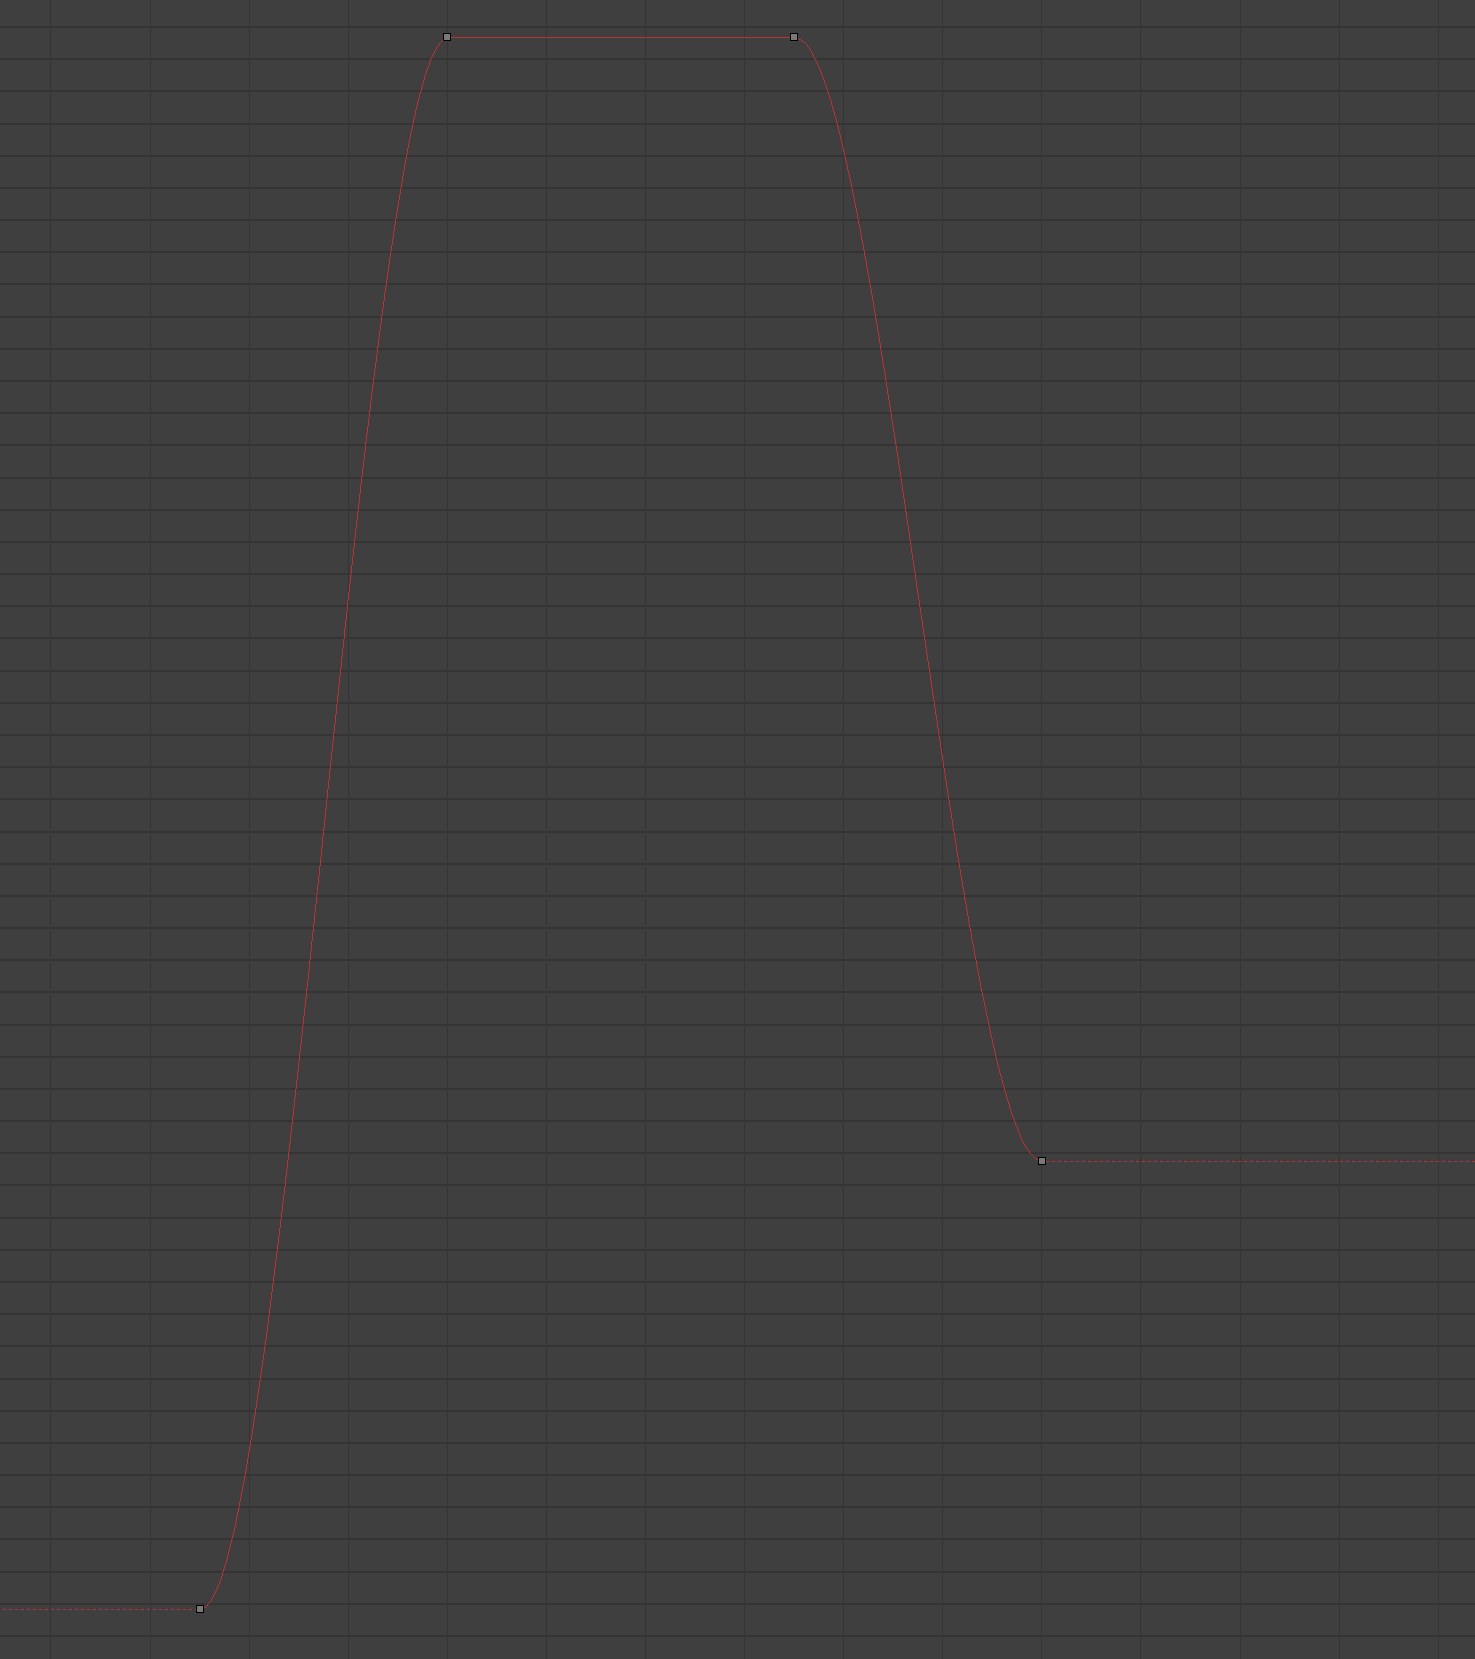
\includegraphics[width=\textwidth]{imagenes/camara/posX.png}
        \caption{Curva de animación de la posición en el eje X con respecto al tiempo.}
    \end{subfigure}
    \hfill
    \begin{subfigure}[t]{0.32\textwidth}
        \centering
        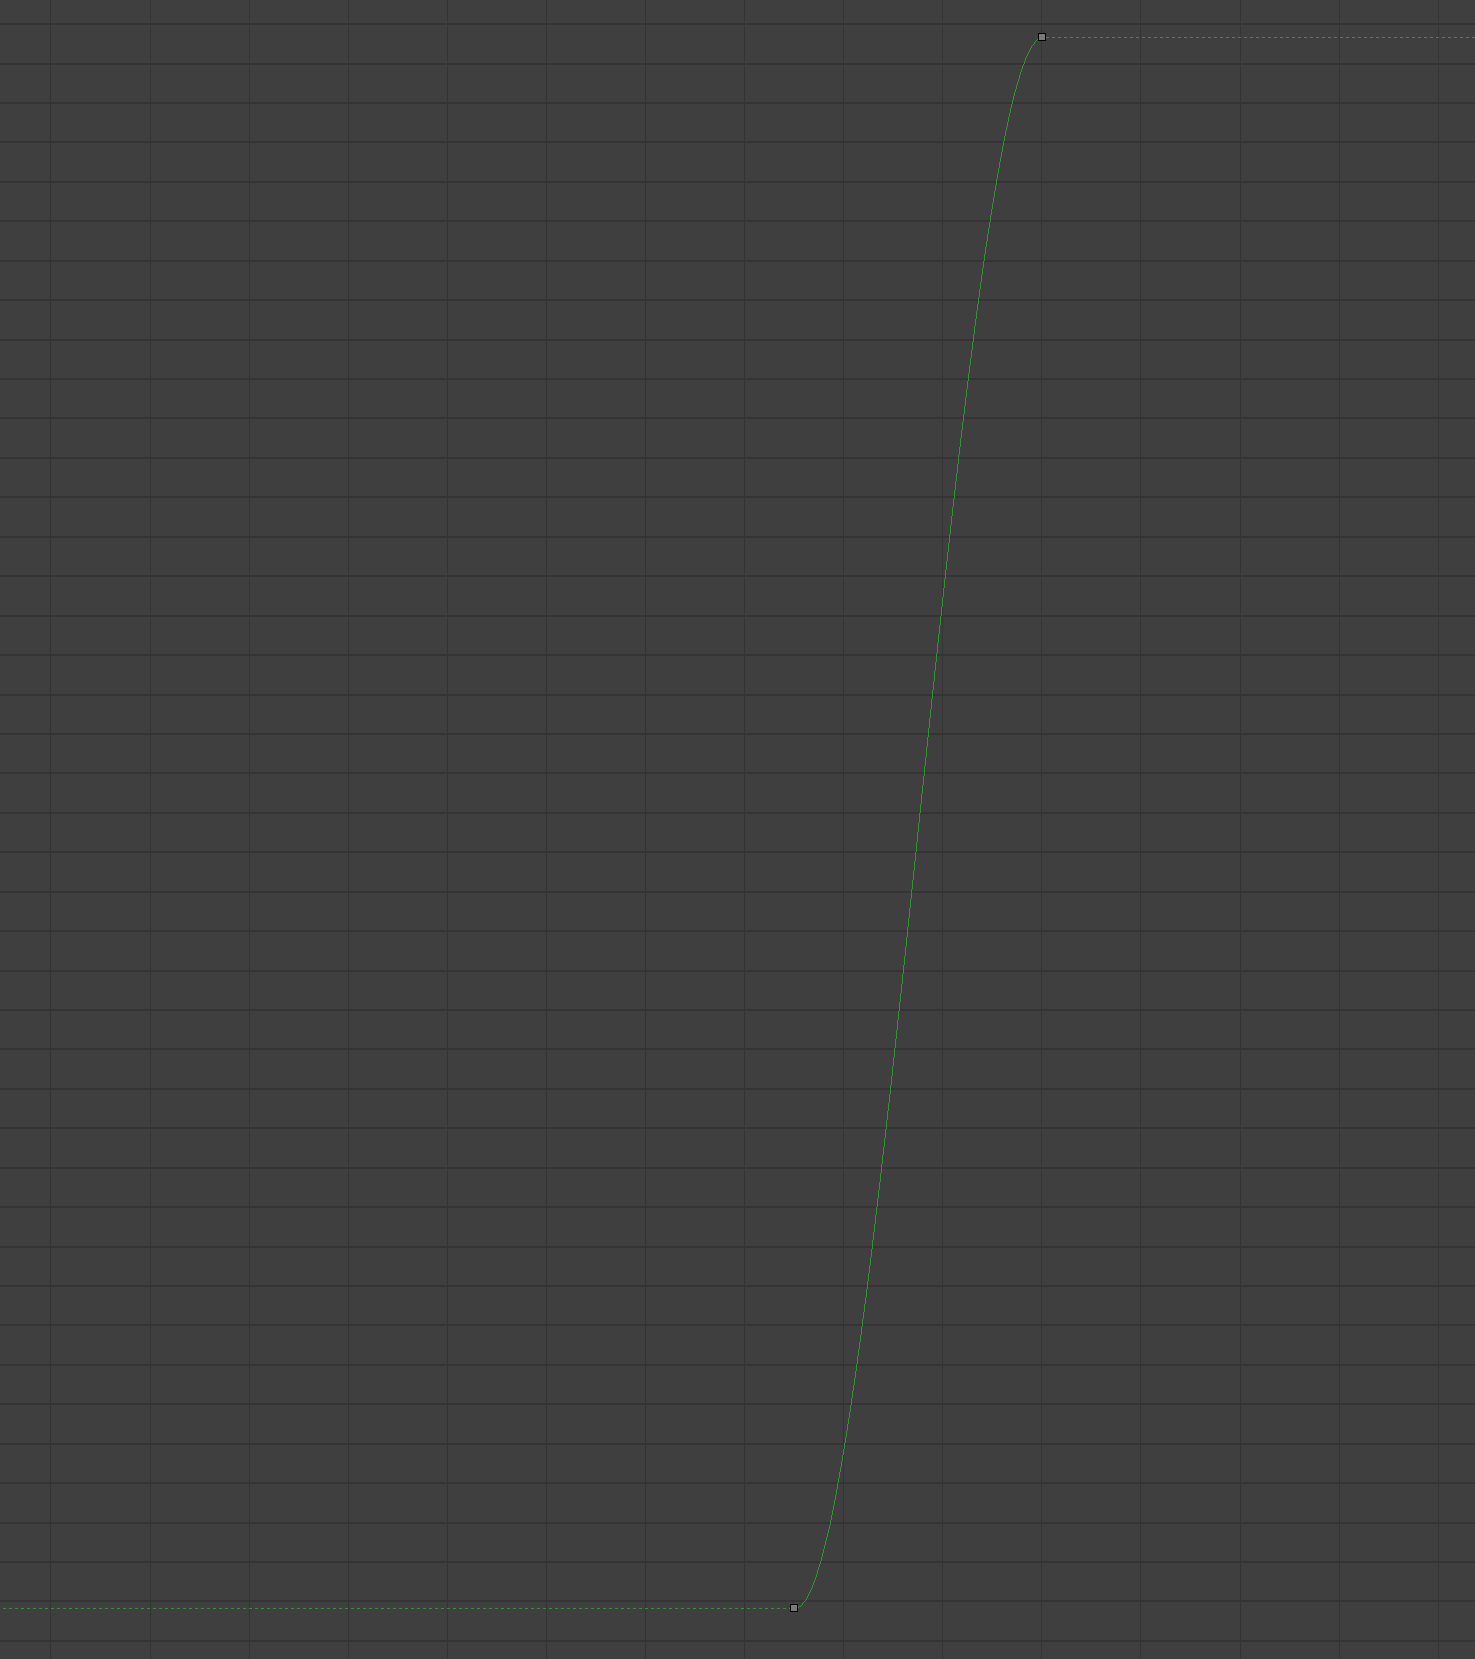
\includegraphics[width=\textwidth]{imagenes/camara/posY.png}
        \caption{Curva de animación de la posición en el eje Y con respecto al tiempo.}
    \end{subfigure}
    \hfill
    \begin{subfigure}[t]{0.32\textwidth}
        \centering
        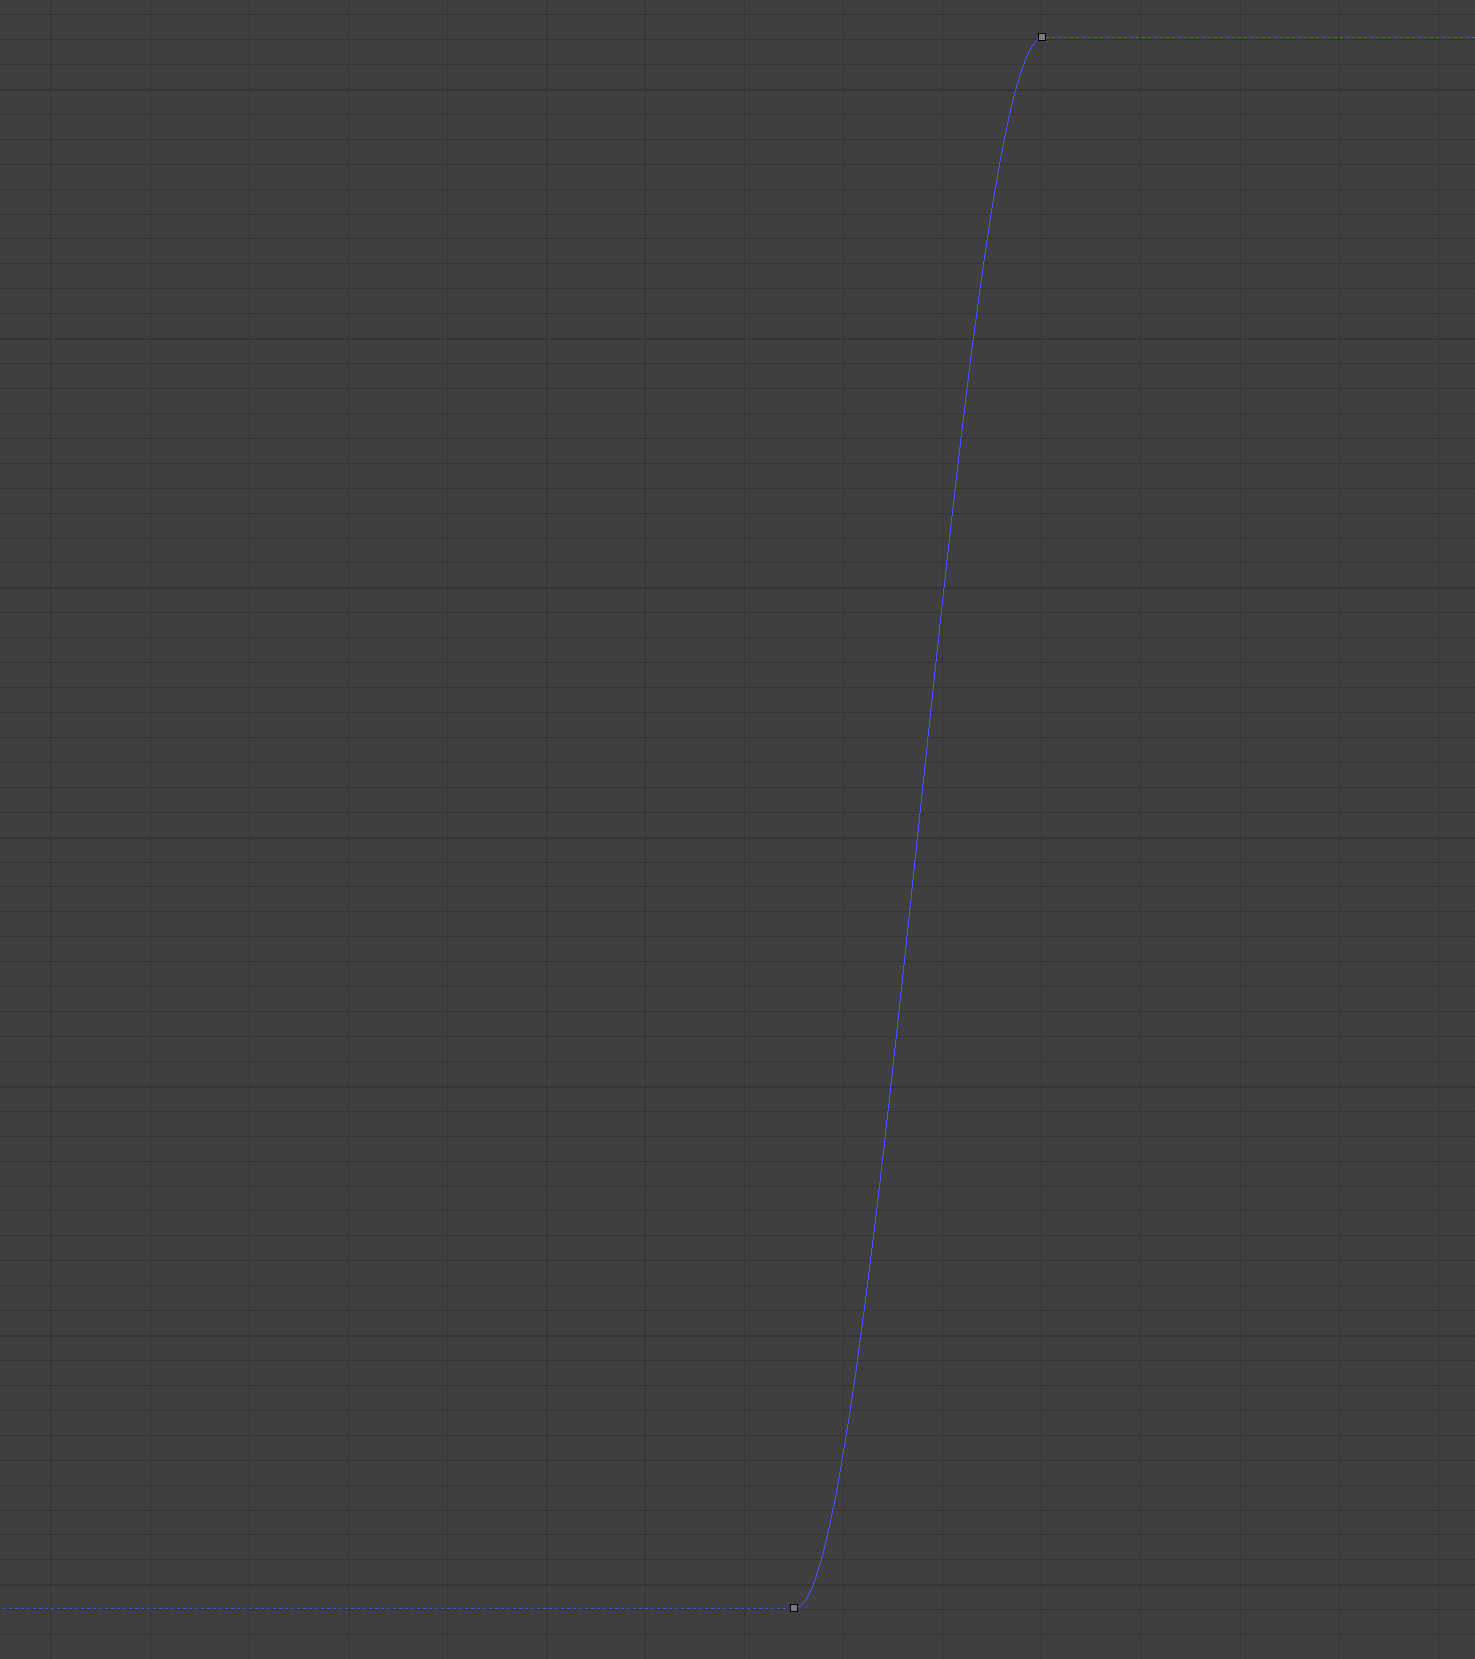
\includegraphics[width=\textwidth]{imagenes/camara/posZ.png}
        \caption{Curva de animación de la posición en el eje Z con respecto al tiempo.}
    \end{subfigure}
    \caption{Curvas de animación para el movimiento de la cámara.}
\end{figure}

% explicacion de las curvas
Como se puede ver, he utilizado la forma de la curva \textit{Slow-in/Slow-out}, ya que es la que me ha parecido que hace un movimiento más suave y realista.

\subsection{Seguimiento de los objetos}

Para realizar el seguimiento de los objetos he utilizado en el \textit{target} de la cámara una restricción de posición (\textit{Position Constraint}), cuyos objetivos son la espada y el coche.

\bigskip

Estos pesos deben cambiar cuando el coche proceda a moverse, para pasar de fijarse en la espada al propio coche. Los \textit{keyframes} de esta restricción son:

\begin{itemize}
    \item \textbf{Instante 125: }El \textit{target} está fijado completamente en la espada y la está siguiendo.
    \item \textbf{Instante 150: }El \textit{target} ahora está fijándose completamente en el coche y lo sigue.
\end{itemize}

\bigskip

En cuanto a las curvas de animación utilizadas, son las siguientes:


\begin{figure}[H]
    \centering
    \begin{subfigure}[t]{0.48\textwidth}
        \centering
        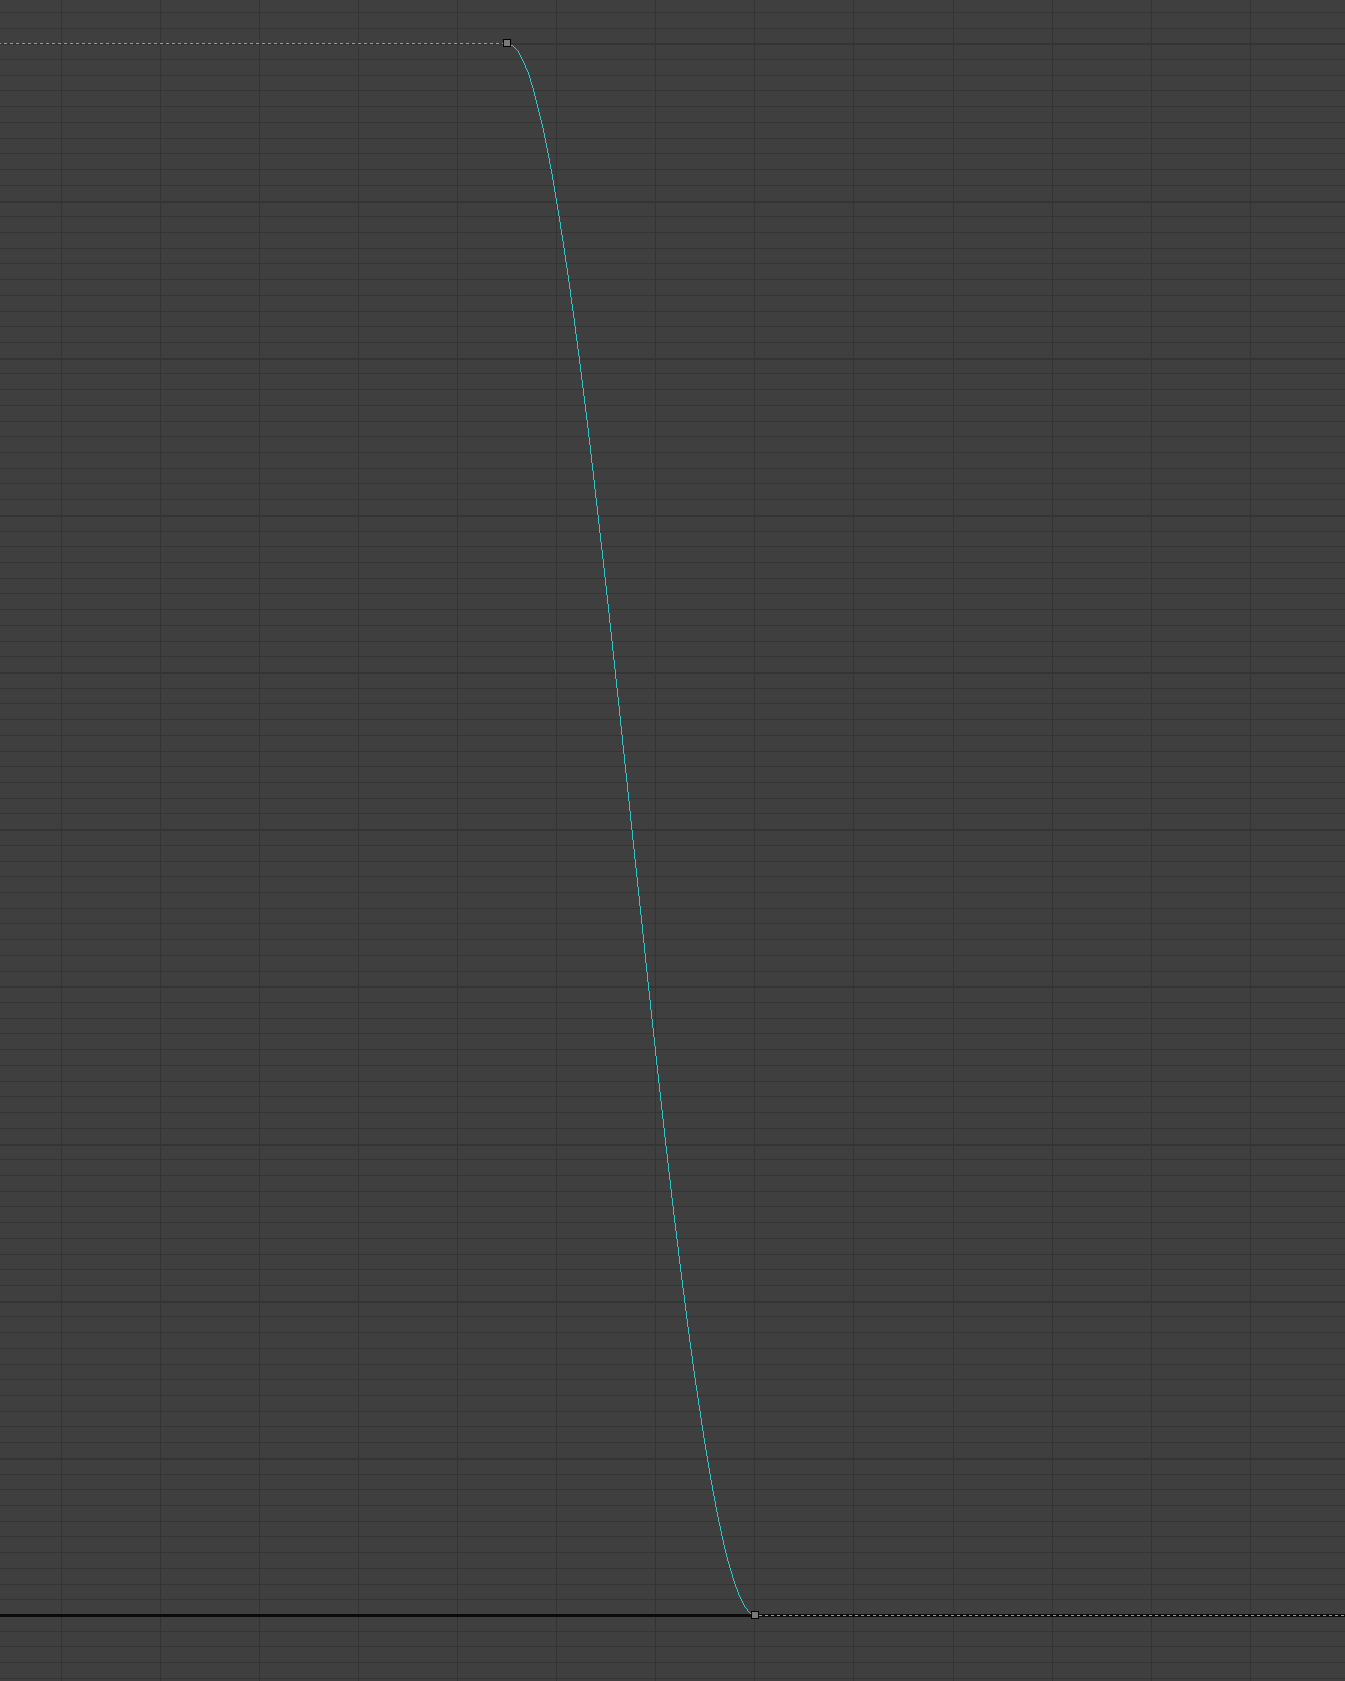
\includegraphics[width=\textwidth]{imagenes/camara/target/pos0.png}
        \caption{Curva de los pesos de la restricción para la espada.}
    \end{subfigure}
    \hfill
    \begin{subfigure}[t]{0.48\textwidth}
        \centering
        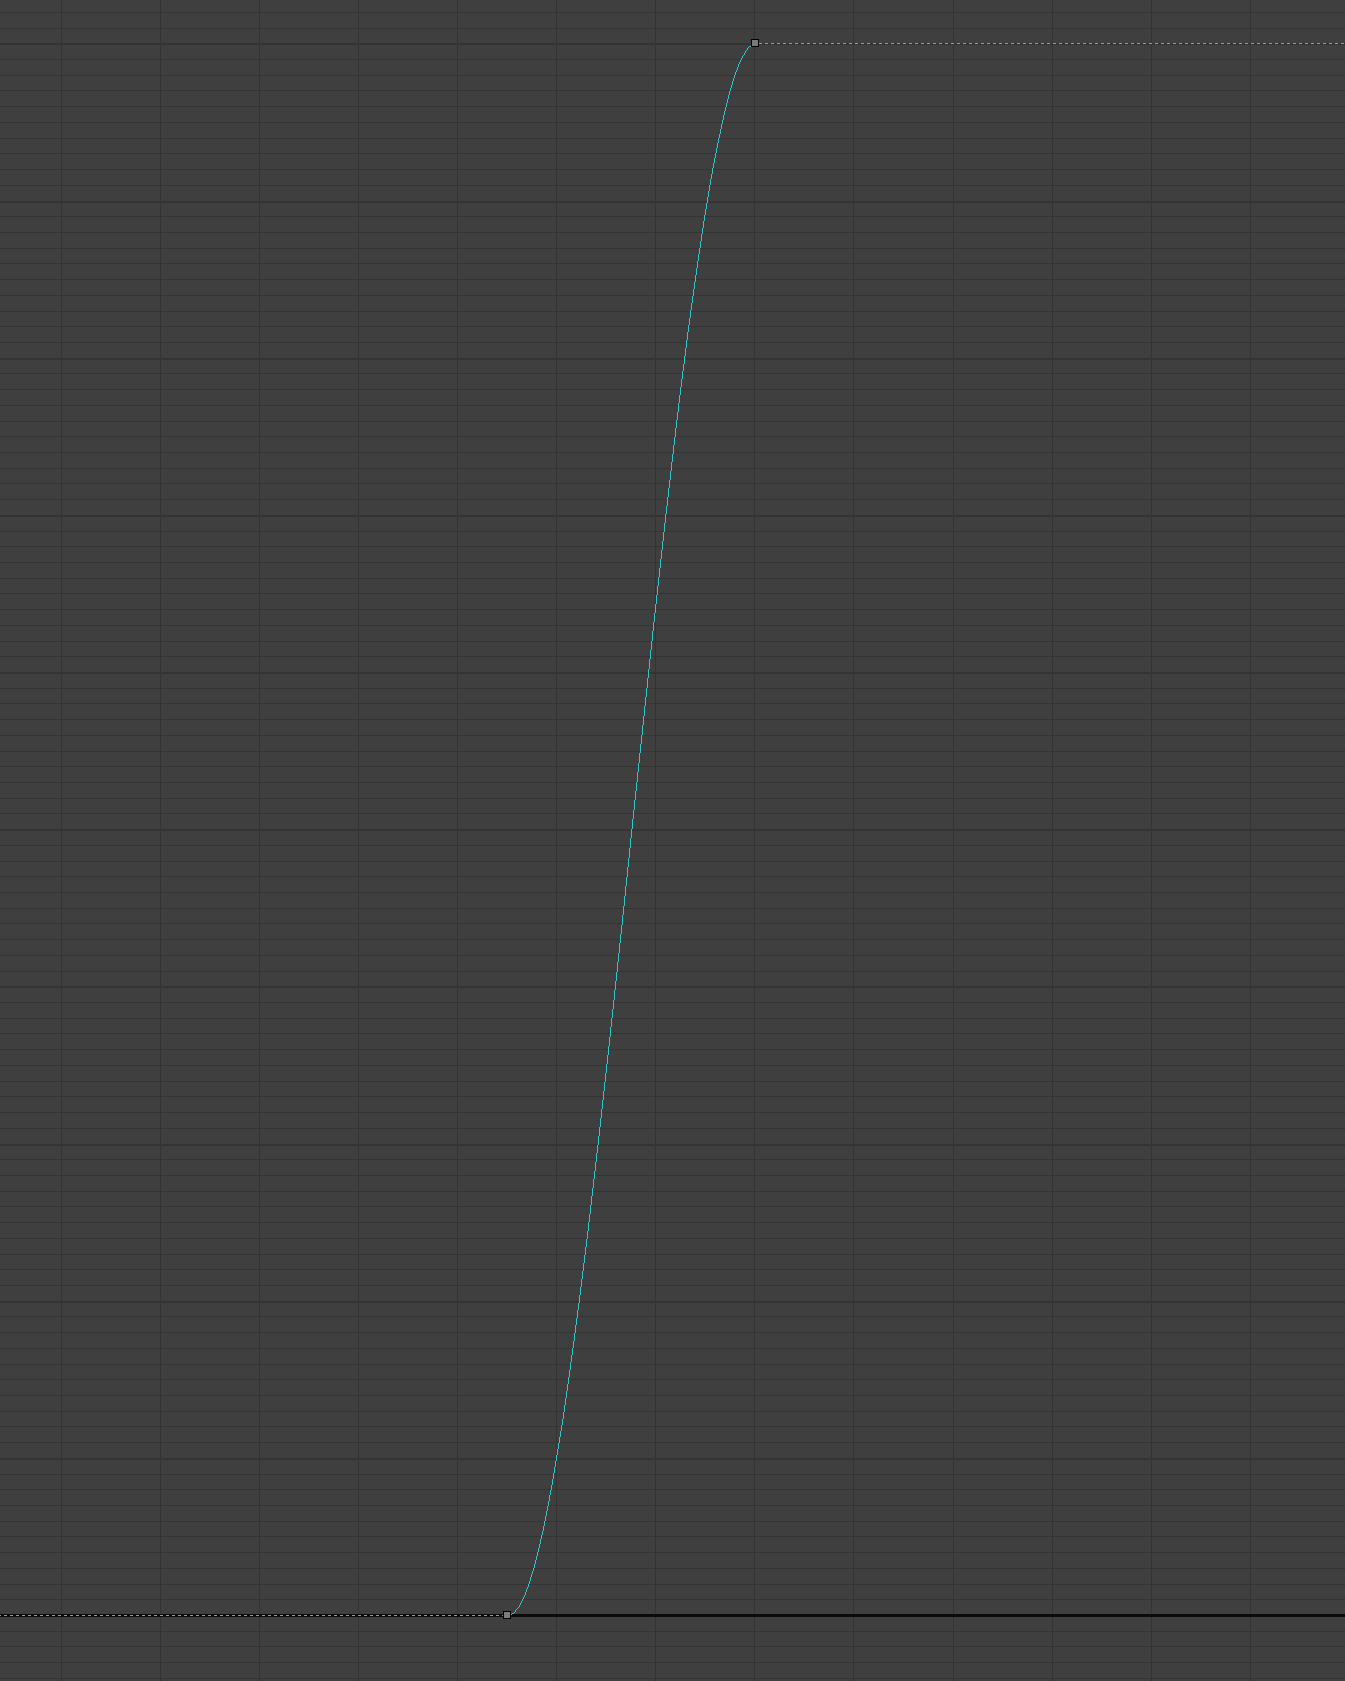
\includegraphics[width=\textwidth]{imagenes/camara/target/pos1.png}
        \caption{Curva de los pesos de la restricción para el \textit{dummy} del coche.}
    \end{subfigure}
    \caption{Curvas de animación para los pesos del \textit{target}.}
\end{figure}

De nuevo, he usado \textit{Slow-in/Slow-out} porque es el que me ha parecido más realista, ya que para mover una cámara de objetivo es necesario hacer un esfuerzo extra al principio, luego pasa a moverse más o menos con la misma velocidad y finalmente hay que aplicar una fuerza en el sentido contrario para pararla. Esto se puede con este tipo de curva.


\subsection{Trayectoria seguida}

La trayectoria seguida por la cámara es la siguiente:

\begin{figure}[H]
    \centering
   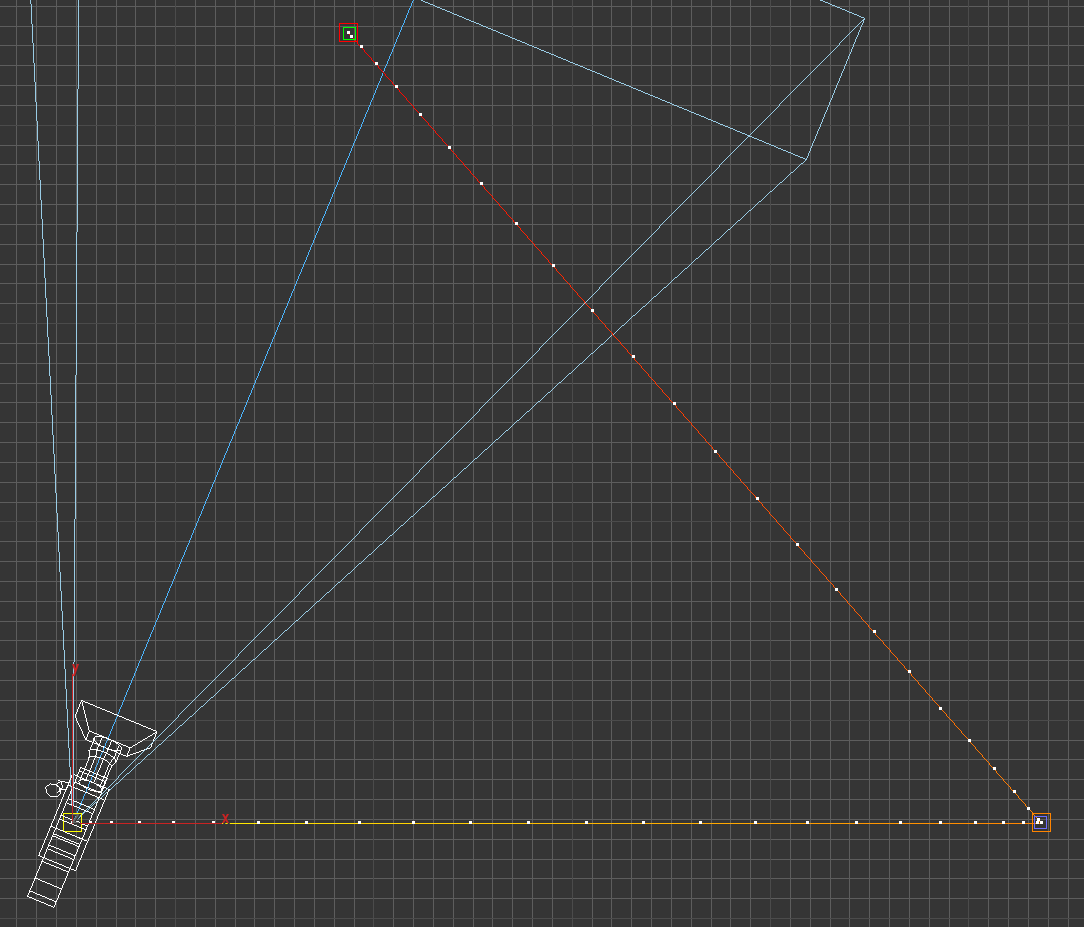
\includegraphics[width=0.6\textwidth]{imagenes/camara/trayectoria.png}
   \caption{Trayectoria seguida por la cámara.}
\end{figure}